\documentclass[a4paper,10pt]{article}
\usepackage[brazilian]{babel}
\usepackage[left=2.5cm,right=2.5cm,top=3cm,bottom=2.5cm]{geometry}
\usepackage{mathtools}
\usepackage{amsthm}
\usepackage{amsmath}
%\usepackage{nccmath}
\usepackage{amssymb}
\usepackage{amsfonts}
\usepackage{physics}
%\usepackage{dsfont}
%\usepackage{mathrsfs}

\usepackage{titling}
\usepackage{indentfirst}

\usepackage{bm}
\usepackage[dvipsnames]{xcolor}
\usepackage{cancel}

\usepackage{xurl}
\usepackage[colorlinks=true]{hyperref}

\usepackage{float}
\usepackage{graphicx}
%\usepackage{tikz}
\usepackage{caption}
\usepackage{subcaption}

%%%%%%%%%%%%%%%%%%%%%%%%%%%%%%%%%%%%%%%%%%%%%%%%%%%

\newcommand{\eps}{\epsilon}
\newcommand{\vphi}{\varphi}
\newcommand{\cte}{\text{cte}}

\newcommand{\N}{\mathbb{N}}
\newcommand{\Z}{\mathbb{Z}}
\newcommand{\Q}{\mathbb{Q}}
\newcommand{\R}{\vb{R}}
\newcommand{\C}{\mathbb{C}}
\renewcommand{\S}{\hat{S}}
%\renewcommand{\H}{\s{H}}

\renewcommand{\a}{\vb{a}}
\newcommand{\nn}{\hat{n}}
\renewcommand{\d}{\dagger}
\newcommand{\up}{\uparrow}
\newcommand{\down}{\downarrow}

\newcommand{\0}{\vb{0}}
%\newcommand{\1}{\mathds{1}}
\newcommand{\E}{\vb{E}}
\newcommand{\B}{\vb{B}}
\renewcommand{\v}{\vb{v}}
\renewcommand{\r}{\vb{r}}
\renewcommand{\k}{\vb{k}}
\newcommand{\p}{\vb{p}}
\newcommand{\q}{\vb{q}}
\newcommand{\F}{\vb{F}}

\newcommand{\s}{\sigma}
%\newcommand{\prodint}[2]{\left\langle #1 , #2 \right\rangle}
\newcommand{\cc}[1]{\overline{#1}}
\newcommand{\Eval}[3]{\eval{\left( #1 \right)}_{#2}^{#3}}

\newcommand{\unit}[1]{\; \mathrm{#1}}

\newcommand{\n}{\medskip}
\newcommand{\e}{\quad \mathrm{e} \quad}
\newcommand{\ou}{\quad \mathrm{ou} \quad}
\newcommand{\virg}{\, , \;}
\newcommand{\ptodo}{\forall \,}
\renewcommand{\implies}{\; \Rightarrow \;}
%\newcommand{\eqname}[1]{\tag*{#1}} % Tag equation with name

\setlength{\droptitle}{-7em}

\theoremstyle{plain}
\newtheorem{theorem}{Teorema}[section]
%\newtheorem{defi}[theorem]{Definição}
\newtheorem{lemma}[theorem]{Lema}
%\newtheorem{corol}[theorem]{Corolário}
%\newtheorem{prop}[theorem]{Proposição}
%\newtheorem{example}{Exemplo}
%
%\newtheorem{inneraxiom}{Axioma}
%\newenvironment{axioma}[1]
%  {\renewcommand\theinneraxiom{#1}\inneraxiom}
%  {\endinneraxiom}
%
%\newtheorem{innerpostulado}{Postulado}
%\newenvironment{postulado}[1]
%  {\renewcommand\theinnerpostulado{#1}\innerpostulado}
%  {\endinnerpostulado}
%
%\newtheorem{innerexercise}{Exercício}
%\newenvironment{exercise}[1]
%  {\renewcommand\theinnerexercise{#1}\innerexercise}
%  {\endinnerexercise}
%
%\newtheorem{innerthm}{Teorema}
%\newenvironment{teorema}[1]
%  {\renewcommand\theinnerthm{#1}\innerthm}
%  {\endinnerthm}
%
\newtheorem{innerlema}{Lema}
\newenvironment{lema}[1]
  {\renewcommand\theinnerlema{#1}\innerlema}
  {\endinnerlema}
%
%\theoremstyle{remark}
%\newtheorem*{hint}{Dica}
%\newtheorem*{notation}{Notação}
%\newtheorem*{obs}{Observação}


\usepackage[shortlabels]{enumitem}

\title{\Huge{\textbf{Lista 3 - Estado Sólido 1}}}
\author{Mateus Marques}

\begin{document}

\maketitle

\section{}

(a) Falso!

\n

Não é verdade que a aproximação do elétron independente leva em consideração o potencial externo de forma completa. Essa aproximação é baseada numa ideia de campo médio, onde as interações elétron-elétron e o potencial dos caroços geram um potencial efetivo que age sobre cada elétron. Dessa maneira, a aproximação de elétron independente ignora os efeitos de muitos-corpos com dependência $(\r_1 - \r_2)$, $(\r_1 - \r_3)$, $(\r_1 - \r_4)$,  $(\r_1 - \r_5)$, $(\r_2 - \r_3)$, $(\r_2 - \r_4)$, etc. Ela leva em conta o potencial externo dos caroços e dos outros elétrons, mas somente de forma aproximada através de um potencial efetivo.

\n\n

(b) Falso!

\n

Embora o Hartree-Fock tente incluir a correlação eletrônica, ele o faz de maneira aproximada através de um campo médio exercido sobre cada elétron e da representação da função de onda como um determinante de Slater. Dessa forma, ele não considera exatamente todos os efeitos de muitos-corpos, que dependem de $(\r_1 - \r_2)$, $(\r_1 - \r_3)$, $(\r_1 - \r_4)$,  $(\r_1 - \r_5)$, $(\r_2 - \r_3)$, $(\r_2 - \r_4)$, etc.

\n\n

(c) Verdadeiro!

\n

No estado fundamental, o último orbital ocupado corresponde ao elétron que necessita de menor energia para ser removido do material. A energia necessária para removê-lo é dada pela diferença entre a energia do estado ionizado e do estado fundamental, que é justamente o autovalor do último orbital ocupado. Portanto, corresponde ao potencial de ionização.

\pagebreak

\section{}

(a) Focalizando a região do gap, a característica principal que distingue os semicondutores é a questão do gap ser direto ou indireto. Examinando cada uma das figuras com cuidado, observando o topo da banda de valência (VBT) e o fundo da banda de condução (CBM), vemos que os semicondutores são dos seguintes tipos.

\begin{itemize}
\item Si: gap indireto.
\item Ge: gap indireto.
\item GaP: gap indireto.
\item GaAs: gap direto.
\item ZnSe: gap direto.
\end{itemize}

\n\n

(b) Quanto ao topo da banda de valência, todos os semicondutores listados possuem portadores do tipo ``buraco'', pois a concavidade é negativa (``para baixo''). Olhando as figuras com bastante paciência, podemos classificar se os portadores são leves ou pesados (subjetivamente) com base em quão agudas são as concavidades do topo da banda de valência (mais agudo significa mais leve).

\begin{itemize}
\item Si: portador tipo ``buraco'' leve.
\item Ge: portador tipo ``buraco'' leve.
\item GaP: portador tipo ``buraco'' pesado.
\item GaAs: portador tipo ``buraco'' pesado.
\item ZnSe: portador tipo ``buraco'' pesado.
\end{itemize}

\n\n

(c) Quanto ao fundo da banda de condução, todos os semicondutores listados possuem portadores do tipo ``elétron'', pois a concavidade é positiva (``para cima''). Olhando as figuras com calma, classificamos se os portadores são leves ou pesados (subjetivamente) com base em quão agudas são as concavidades do fundo da banda de condução.

\begin{itemize}
\item Si: portador tipo ``elétron'' pesado.
\item Ge: portador tipo ``elétron'' pesado.
\item GaP: portador tipo ``elétron'' pesado.
\item GaAs: portador tipo ``elétron'' leve.
\item ZnSe: portador tipo ``elétron'' leve.
\end{itemize}

\n\n

(d) A principal diferença entre a estrutura de bandas do ZnSe para os demais é que a banda de valência não é degenerada, igual aos demais que sempre possuem degenerescência no trecho $\Gamma \to X$. Essa separação da degenerescência (``splitting'') provavelmente ocorre devido à uma interação spin-órbita, que é relevante para o material ZnSe.

\pagebreak

\section{}

(a) A Densidade de Estados (DOS) $D(E)$ é definida de maneira que $D(E) \dd{E}$ seja o número de estados eletrônicos que possuem energia entre $E$ e $E + \dd{E}$. Ela é usada para compreender o comportamento eletrônico dos materiais e é útil para determinar, por exemplo, a condutividade elétrica e susceptibilidade magnética.

\n\n

A Densidade Conjunta de Estados (JDOS) é uma generalização da DOS que leva em consideração a interação entre diferentes estados, usando duas ou mais variáveis como a energia ou momento. Ela é utilizada na caracterização de processos de excitação, como transições eletrônicas e absorção de fótons. Em aula, vimos que ela é extremamente útil para estudar os processos ópticos nos materiais na região da luz visível.

\n\n

(b) No caso de um semicondutor de gap direto (GaAs), o gap óptico coincide com o gap eletrônico, já que as transições verticais da VBT para CBM (aproximamos $\Delta k \approx 0$ devido a considerarmos luz visível) são permitidas.

\begin{figure}[H]
\centering
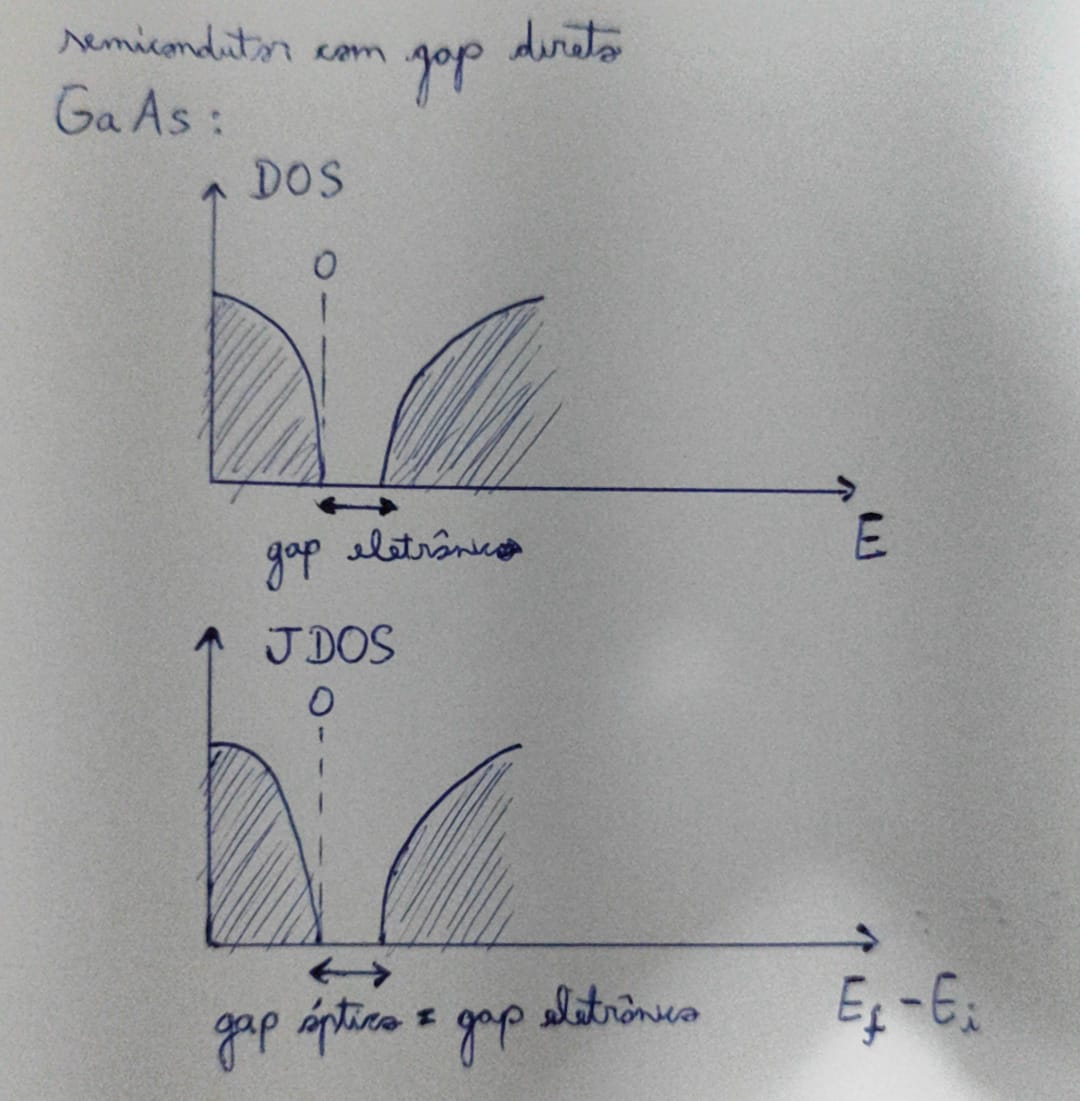
\includegraphics[width=0.38\linewidth]{fig/dos-jdos-direto.jpeg}
\caption{Esboço da DOS e JDOS para um semicondutor de gap direto (GaAs).}
\label{fig:dos-jdos-direto}
\end{figure}


\n

(c) No caso de um semicondutor de gap indireto (Si), o gap óptico é naturalmente maior que o gap eletrônico, já que as transições verticais da VBT para CBM não são permitidas. Somente em energias maiores as transições verticais acontecem no processo óptico de absorção.

\begin{figure}[H]
\centering
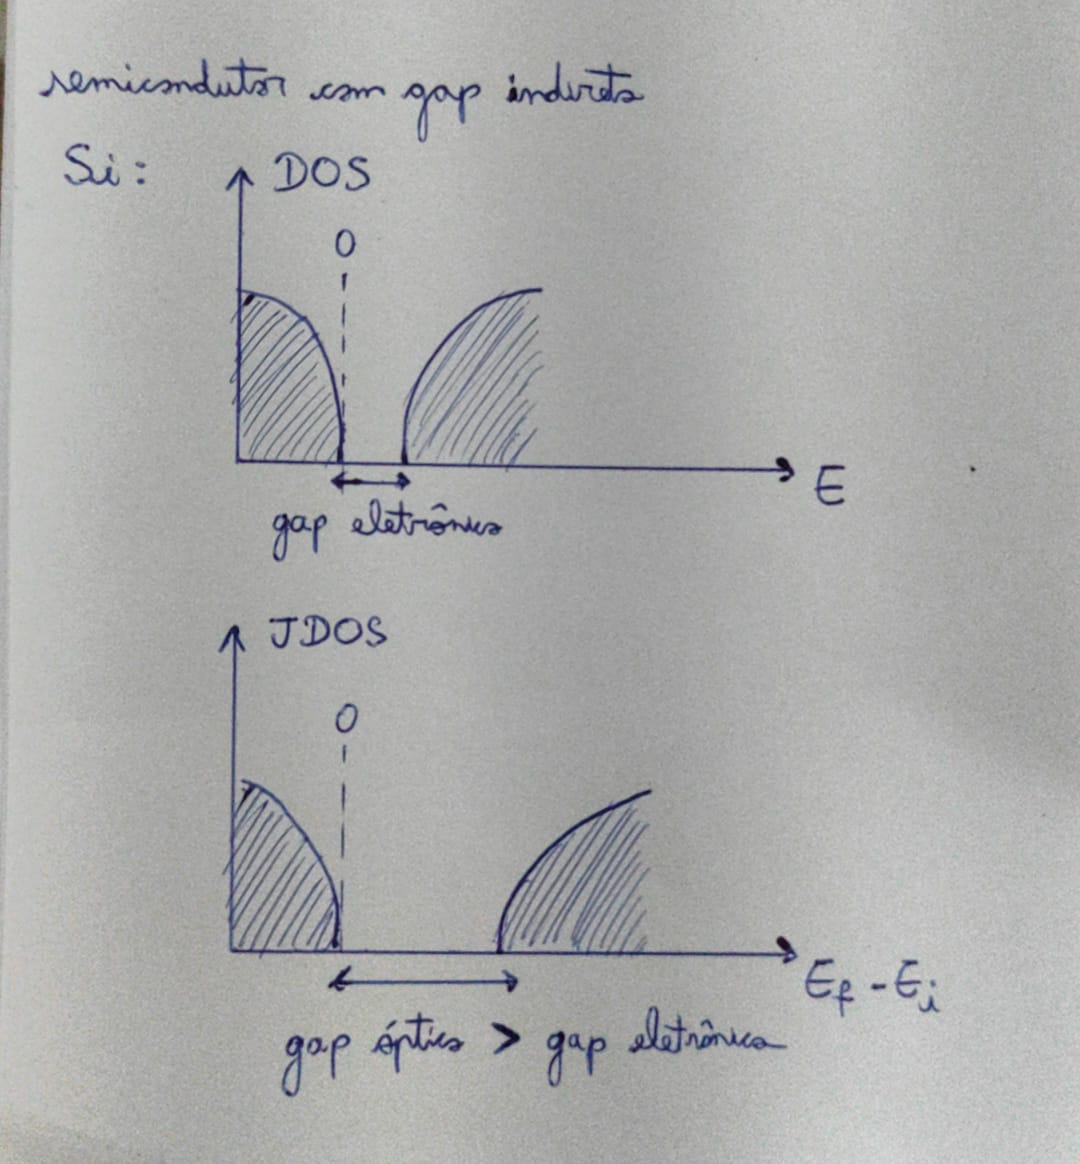
\includegraphics[width=0.38\linewidth]{fig/dos-jdos-indireto.jpeg}
\caption{Esboço da DOS e JDOS para um semicondutor de gap indireto (Si).}
\label{fig:dos-jdos-indireto}
\end{figure}

\n

(d) Para aplicações ópticas que dependem da absorção de energia da luz, semicondutores de gap direto (GaAs) são mais adequados. Isso ocorre porque o gap óptico é menor, o que implica em absorções mais eficientes.

Para semicondutores de gap indireto (Si), a transição entre a banda de valência e a banda de condução envolve um momento maior do fóton incidente. Isso torna a absorção de fótons menos eficiente e requer uma energia maior no processo.

\pagebreak

\section{}

(a) A expressão da equação \ref{eq:potquim} é bastante simplificada e envolve diversas aproximações.
\begin{equation} \label{eq:potquim}
\mu_i = \frac{1}{2} (E_c + E_v) + \frac{3}{4} k_B T \ln(\frac{m_{hh}^*}{m_c^*}).
\end{equation}

Primeiramente, é assumido que a concentração de portadores de carga no semicondutor intrínseco é devida somente aos efeitos da temperatura. Agora, dentre as aproximações envolvidas, assume-se que em temperatura zero o nível de Fermi está exatamente no meio do gap entre a banda de valência e a banda de condução e também é utilizado um modelo simplificado para a DOS (baseado na dispersão de partícula livre) dos elétrons (com massa efetiva $m_c^*$ na banda de condução) e dos buracos (com massa efetiva $m_{hh}^*$ na banda de valência). Além disso, para derivar a equação \ref{eq:potquim}, também assume-se que a temperatura seja suficientemente pequena de maneira que $\displaystyle{\frac{1}{e^{\beta(E-\mu)} + 1} \approx e^{-\beta(E-\mu)}}$.

\n\n

(b) Na derivação da equação \ref{eq:potquim}, o fato do gap ser direto ou indireto não é relevante pois não há menção explícita do momento. Dessa maneira, a equação \ref{eq:potquim} vale tanto para o Si (gap indireto) quanto para o GaAs (gap direto).

\n\n

(c) Na tabela 4.1 e no problema 3.18 do livro ``Semiconductor Physics and Devices'' \cite{neamen}, obtemos os dados correspondentes ao Si e ao GaAs na temperatura $T = 300 \unit{K}$. Também assumirei que $E_v = 0 \unit{eV}$ (convenção da energia de Fermi no zero) e o valor da constante $k_B = 8.617 \cdot 10^{-5} \unit{eV/K}$.
\begin{itemize}
\item Si à $T = 300 \unit{K}$: $E_g = 1.12 \unit{eV}$, $m_c^* = 1.08 \, m_0$, $m_{hh}^* = 0.56 \, m_0$. Fazendo o cálculo com esses dados do Si, obtemos
$$
\boxed{\mu_{\text{Si}, \; 300\unit{K}} = 0.55 \unit{eV}.}
$$

\n

\item GaAs à $T = 300 \unit{K}$: $E_g = 1.42 \unit{eV}$, $m_c^* = 0.067 \, m_0$, $m_{hh}^* = 0.48 \, m_0$. Fazendo o cálculo com esses dados do GaAs, obtemos
$$
\boxed{\mu_{\text{GaAs}, \; 300\unit{K}} = 0.75 \unit{eV}.}
$$
\end{itemize}



%%-----
%% Referências bibliográficas
%%-----
\addcontentsline{toc}{chapter}{\bibname}
%\bibliographystyle{abntex2-num}
\bibliography{citations}
\bibliographystyle{ieeetr}


\end{document}
